%%%%%%%%%%%%%%%%%%%%%%%%%%%%%%%%%%%%%%%%%%%%%%%%%%%%%%%%%%%%%%%%%%
%%%%%%%% ICML 2014 EXAMPLE LATEX SUBMISSION FILE %%%%%%%%%%%%%%%%%
%%%%%%%%%%%%%%%%%%%%%%%%%%%%%%%%%%%%%%%%%%%%%%%%%%%%%%%%%%%%%%%%%%

% Use the following line _only_ if you're still using LaTeX 2.09.
%\documentstyle[icml2014,epsf,natbib]{article}
% If you rely on Latex2e packages, like most moden people use this:
\documentclass{article}

% use Times
\usepackage{times}
% For figures
\usepackage{graphicx} % more modern
%\usepackage{epsfig} % less modern
\usepackage{subfigure}

% For citations
\usepackage{natbib}

% For algorithms
\usepackage{algorithm}
\usepackage{algorithmic}

% As of 2011, we use the hyperref package to produce hyperlinks in the
% resulting PDF.  If this breaks your system, please commend out the
% following usepackage line and replace \usepackage{icml2014} with
% \usepackage[nohyperref]{icml2014} above.
\usepackage{hyperref}

% Packages hyperref and algorithmic misbehave sometimes.  We can fix
% this with the following command.
\newcommand{\theHalgorithm}{\arabic{algorithm}}

% Employ the following version of the ``usepackage'' statement for
% submitting the draft version of the paper for review.  This will set
% the note in the first column to ``Under review.  Do not distribute.''
\usepackage{icml2014} 


% The \icmltitle you define below is probably too long as a header.
% Therefore, a short form for the running title is supplied here:
\icmltitlerunning{Objected Recognition based on learning}

\begin{document} 

\twocolumn[
\icmltitle{Objects Recognization Based on On-line Machine Learning\\Project Status Report for CIS 519}

% It is OKAY to include author information, even for blind
% submissions: the style file will automatically remove it for you
% unless you've provided the [accepted] option to the icml2014
% package.
\icmlauthor{Shangyi Cheng}{shangyi@seas.upenn.edu}
\icmlauthor{Yao Chu}{chuyao@seas.upenn.edu}
\icmlauthor{Chenyang Zhao}{chzhao@seas.upenn.edu}

% You may provide any keywords that you 
% find helpful for describing your paper; these are used to populate 
% the "keywords" metadata in the PDF but will not be shown in the document
\icmlkeywords{machine learning, circle detection, feature extraction, objects recognization, neural network}

\vskip 0.3in
]

\begin{abstract} 
So far, we attempted to use following method described in this report to recognize objects (various kinds of balls in our project) in the given images. The first step is using Circular Hough Tansform (CHT) to detect the most possible region that contains the ball which is datasets preprocessing step. The second step contains techniques to extract feature from the selected region. In the third step, neural network is applied on the extracted features to classify the given instances. Several training/testing experiments have be carried out to show the performance of this method.
\end{abstract}


\section{Introduction}

This report presents an attempt of objects recognition. We decided to use images of four kinds of balls from Caltech 256(Griffin, G. Holub, AD. Perona, P.) as our dataset, which contains 98 images of golf in the folder ``088.golf-ball'', 174 in ``193.soccer-ball'', 104 in ``017.bowling-ball'' and 98 in ``216.tennis-ball''.\\
Primary tasks for this project:
\begin{enumerate}
\item Preprocess the datasets and extract the picture patches with different labels. So far, CHT was applied to test the geometric feature of the balls.
\item Based on machine learning method (e.g. Neural Network) to train the datasets.
\item In the test part, input a test image, the algorithm should detect balls in the image and label the detected ball based on the trained model. 
\end{enumerate}

\section{SVM learning}
Support vector machine(SVM) is one of basic learning algorithm that most widely used to solve object recognition problems \cite{HogDetection1},\cite{SVMforRecogintion}. In our case, we applied one-class SVM first and extend it to multi-class to train the dataset with several different labels.
\subsection{One-Class SVM}
Given a set of instances which belongs to either of two classes, a SVM classifier finds the optimal hyperplane leaving the largest possible fraction of instances of the same class on the same side, while maximize the distance of either class from hyperplane, by maximize the $J(\alpha)$ in \ref{eq:Jfunc}.
\begin{equation}
J(\alpha) = \sum_{i=1}^n \alpha_i - \frac{1}{2}\sum_{i=1}^n\sum_{j=1}^n \alpha_i \alpha_jy_iy_j\langle x_i,x_j\rangle
\label{eq:Jfunc}
\end{equation}
s.t. $\alpha_i\leq 0 \forall i$, $\sum_i \alpha_iy_i = 0$,
where $\alpha_i$ is the constraints weight scaler, and $\langle x_i,x_j \rangle$ is a scaler given by the kernel function.\\
While applying SVM algorithm, choosing proper kernel is essential to train the classifier. We used two different kernels to train the dataset, which are Gaussian kernel, linear kernel, and drew the Receiver	Operating Characteristic(ROC) curve respectively. The result are shown in the figure (\ref{fig:ROC}). As shown in the figure, the Gaussian kernel gives better prediction.\\
\begin{figure}[htb]
\centering
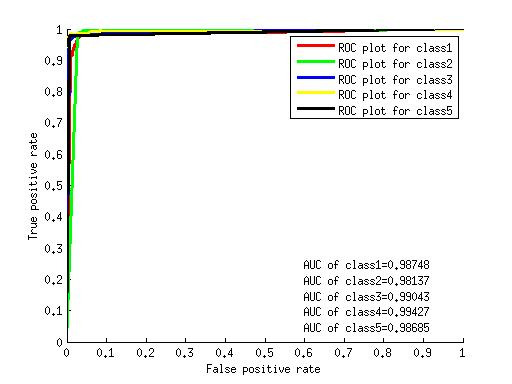
\includegraphics[width = 0.4\textwidth]{ROCgauss.jpg}
\end{figure}

\begin{figure}[htb]
\centering
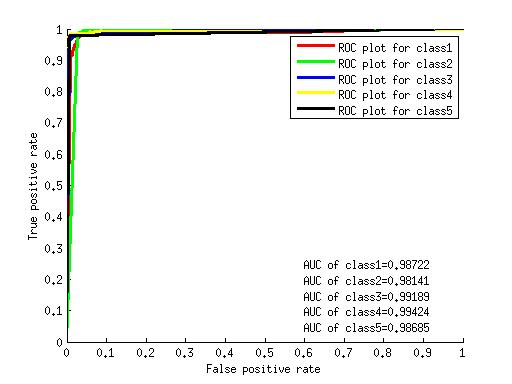
\includegraphics[width = 0.4\textwidth]{ROClinear.jpg}
\end{figure}
\subsection{Multi-Class SVM}
Traditional SVM algorithm only solves 2-classes problems. However, detecting ball object in a image should be able to tell whether there is a ball and figure out the type of the ball object, which is a multi-class classification problem. Therefore, one-vs-rest is introduced for solving multi-class problem.\\
Given a dataset with $k$ different labels, $k$ different one-class SVM classifiers is trained for each class. When training for individual class, the instances that belongs to this class are labeled as $1$, and all the others are labeled as $0$. A new instance should be predicted as in the class which gives the largest scores value.\\
\subsection{Grid Search}

\section{result}
\subsection{Learning Curve}
To evaluate our SVM classifier, we run our classifier through 10-fold cross validation and drew the learning curve in figure (\ref{fig:learning curve}) to show the performance versus the number of training examples. 


\section*{Acknowledgments}
This project is supported by Upenn CIS 519. Thanks Eric Eaton and Xiaoxiang Hu for their instruction. Thanks MATLAB for providing some many useful toolbox.

\bibliography{status-ChengChuZhao}
\bibliographystyle{icml2014}

\end{document} 


